\documentclass{article}

\usepackage[final,main,nonatbib]{neurips_2026}
\usepackage[UTF8,heading=false]{ctex}
\usepackage{amsmath}
\usepackage{amssymb}
\usepackage{booktabs}
\usepackage{graphicx}
\usepackage{float}
\usepackage{hyperref}

\graphicspath{{../outputs/}{../outputs/figs/}{project/outputs/}{project/outputs/figs/}{MRI_projects/T1_MRI_denoising/outputs/}{MRI_projects/T1_MRI_denoising/outputs/figs/}}

\title{基于 2.5D Residual U-Net 的 T1 MRI 去噪}

\author{}

\begin{document}
\maketitle

\begin{center}
\small
\textbf{GitHub 仓库：}\url{https://github.com/yvepan/Computational-Neuroscience-project}\\
\textbf{模型权重：}\url{https://drive.google.com/file/d/1GytKqEMeoEHM6e87vdCDSrrdNKzpEPVe/view?usp=drive_link}
\end{center}

\begin{abstract}
本实验实现 T1 MRI 从加噪图像到干净图像的监督式去噪。数据集包含 600 个病例，体积尺寸不固定，并包含 Gaussian 与 Rician 混合噪声。为避免信息泄漏，病例划分固定为 480/60/60，脑掩膜和归一化参数仅由 noisy 图像估计，clean 图像只作为训练标签和评估真值。主方法采用 2.5D Residual 2D U-Net，以相邻 axial 切片作为 3 通道输入，并预测噪声残差而非直接预测 clean 图像。在 60 个测试病例上，该方法达到 PSNR $43.01\pm1.82$ dB、SSIM $0.9959\pm0.0015$，相对 noisy 输入提升 1.25 dB PSNR，并在所有测试病例上优于 Gaussian smoothing 与 NLM 基线。
\end{abstract}

\section{数据与预处理}

本实验选择 T1 MRI 去噪任务。每个病例包含 \texttt{T1\_noisy.nii.gz} 与 \texttt{T1\_clean.nii.gz}。实测体积尺寸范围约为 $156$--$208 \times 203$--$256 \times 166$--$256$，因此代码不假设固定尺寸。所有图像为 RAS 朝向、1 mm 各向同性体素，axial 切片沿第 3 轴。

数据按病例而非切片划分，固定随机种子为 42，得到 480 个训练病例、60 个验证病例和 60 个测试病例，并写入 \texttt{split.json}。所有脚本读取同一划分文件，以避免切片级泄漏。

预处理只使用 noisy 图像估计脑掩膜和归一化参数。脑掩膜由 Gaussian 平滑、Otsu 阈值、形态学清理和最大连通域筛选得到。归一化使用 noisy 脑区第 1 和第 99.5 百分位作为 $(lo, hi)$，并对 noisy 与 clean 共用：
\begin{equation}
  \hat{x}=\frac{x-lo}{hi-lo}, \qquad \hat{y}=\frac{y-lo}{hi-lo}.
\end{equation}
这保证 clean 图像不参与输入侧统计量估计。预处理结果缓存为 \texttt{.npz}，训练时仅采样脑区占比超过 1\% 的 axial 切片。

\section{方法}

训练样本由中心 axial 切片及其前后相邻切片组成：
\begin{equation}
  X_k=[x_{k-1},x_k,x_{k+1}]\in\mathbb{R}^{3\times H\times W}.
\end{equation}
标签为 clean 的中心切片 $y_k$。训练阶段随机裁剪 $192\times192$ patch，并使用水平和垂直翻转增强。验证和测试阶段对整张切片推理，先 padding 到 16 的倍数，再裁回原尺寸。

模型为 Residual 2D U-Net，输入通道数为 3，输出通道数为 1，base channel 为 48，共 4 层下采样。每个 stage 使用残差卷积块，上采样采用双线性插值。网络预测噪声残差 $r_\theta(X_k)$，最终输出为
\begin{equation}
  \hat{y}_k=x_k-r_\theta(X_k).
\end{equation}
该设计将学习目标集中在 noisy 与 clean 的差异上，更符合去噪任务。

损失函数为
\begin{equation}
  \mathcal{L}
  =\|\hat{y}-y\|_1
  +0.2(1-\mathrm{SSIM}(\hat{y},y))
  +0.1\mathcal{L}_{grad}.
\end{equation}
其中 SSIM 的 \texttt{data\_range} 固定为 1.0，梯度损失使用 Sobel 梯度图的 L1 距离，用于降低过平滑。

\section{训练设置与断点续传}

训练使用 AdamW，学习率 $10^{-4}$，weight decay $10^{-4}$，batch size 16，最大 60 epoch，并启用 AMP 混合精度。每个 epoch 后在 60 个验证病例上做整卷推理，以脑掩膜内 PSNR 选择最优模型。

断点续传保存两类 checkpoint：\texttt{last.pt} 与 \texttt{best.pt}。\texttt{last.pt} 包含模型、优化器、scheduler、AMP scaler、epoch、global step、best PSNR、early stopping 计数、随机状态和配置；\texttt{best.pt} 在验证 PSNR 刷新时保存。保存过程先写临时文件，再用 \texttt{os.replace} 原子替换目标文件。训练脚本启动时默认从 \texttt{last.pt} 续训，只有显式指定 \texttt{--resume none} 才从头训练。为减少 I/O 开销，最终配置不按 step 保存，而是每 2 epoch 保存一次中间状态，同时保留 best checkpoint。

最终训练到 epoch 60。最佳验证结果也出现在 epoch 60，验证 PSNR 为 43.0978 dB，验证 SSIM 为 0.9960。训练曲线如图~\ref{fig:curves} 所示。

\begin{figure}[H]
  \centering
  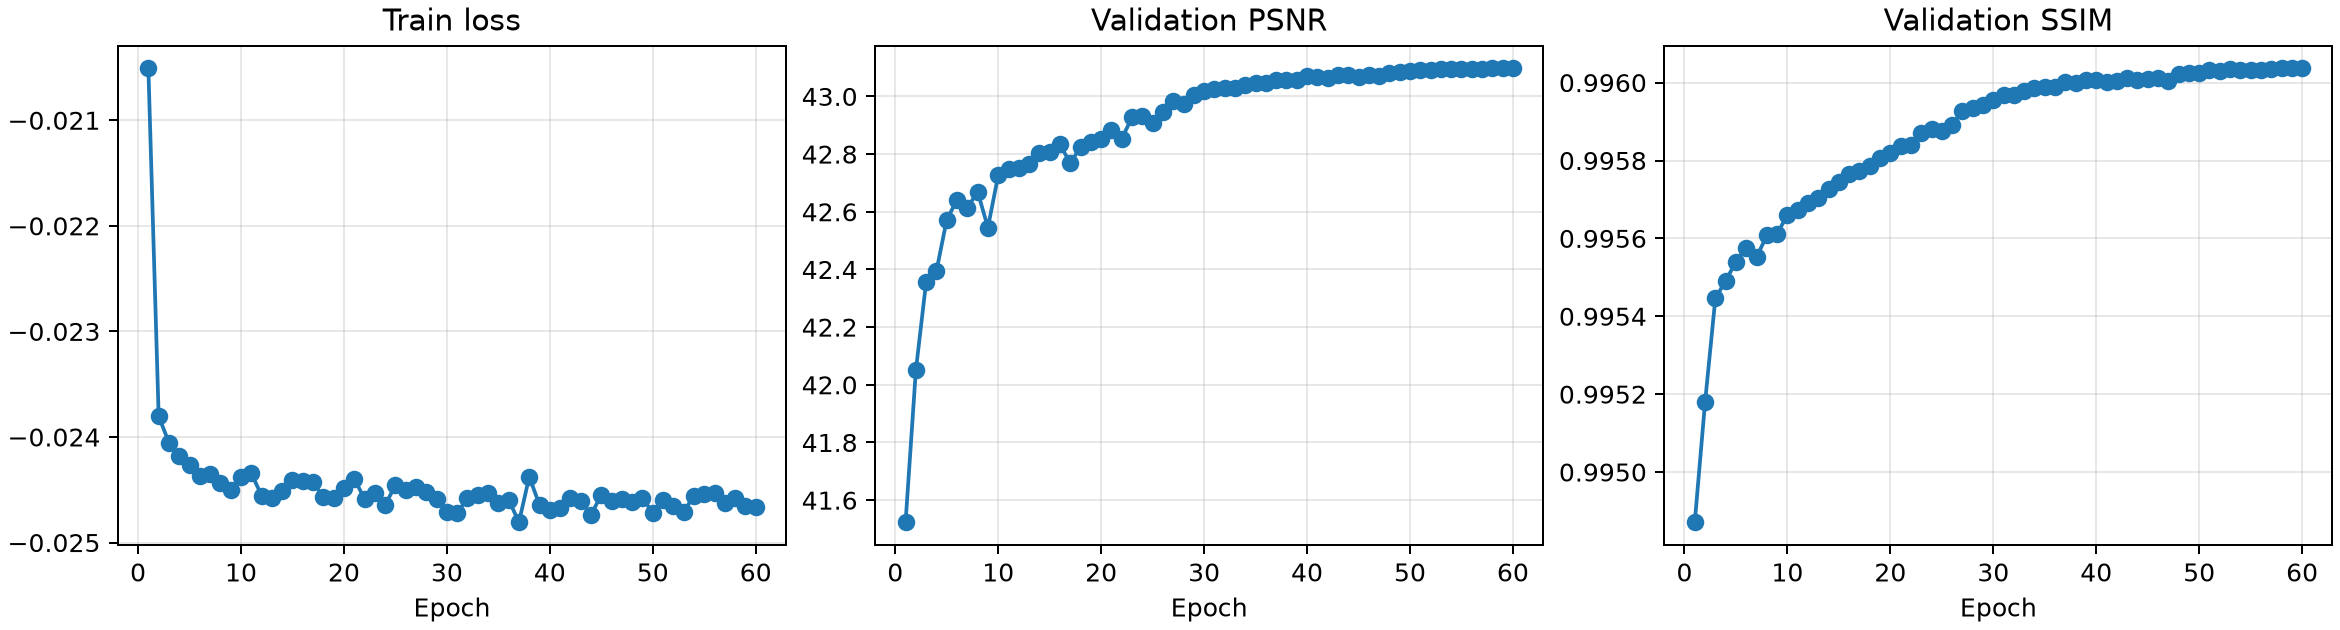
\includegraphics[width=0.86\linewidth]{training_curves.png}
  \caption{训练损失、验证 PSNR、验证 SSIM 与学习率曲线。}
  \label{fig:curves}
\end{figure}

\section{结果}

评估在 60 个测试病例上进行。所有指标只在 noisy 推导出的脑掩膜内统计，预测结果先 clip 到 $[0,1]$，并固定 \texttt{data\_range=1.0}。比较方法包括 Noisy、Gaussian smoothing、NLM 和 Residual U-Net。

\begin{table}[H]
  \centering
  \caption{测试集整体结果（mean $\pm$ std）。MAE/RMSE 越低越好，PSNR/SSIM 越高越好。}
  \label{tab:main}
  \small
  \begin{tabular}{lcccc}
    \toprule
    Method & MAE $\downarrow$ & RMSE $\downarrow$ & PSNR $\uparrow$ & SSIM $\uparrow$ \\
    \midrule
    Gaussian & $0.0091\pm0.0009$ & $0.0125\pm0.0010$ & $38.09\pm0.66$ & $0.9932\pm0.0019$ \\
    NLM & $0.0066\pm0.0015$ & $0.0084\pm0.0019$ & $41.77\pm2.05$ & $0.9937\pm0.0026$ \\
    Noisy & $0.0067\pm0.0016$ & $0.0084\pm0.0020$ & $41.76\pm2.15$ & $0.9936\pm0.0029$ \\
    \textbf{Residual U-Net} & $\mathbf{0.0057\pm0.0011}$ & $\mathbf{0.0072\pm0.0014}$ & $\mathbf{43.01\pm1.82}$ & $\mathbf{0.9959\pm0.0015}$ \\
    \bottomrule
  \end{tabular}
\end{table}

Residual U-Net 在全部指标上优于三种基线。PSNR 相比 Noisy 提升 1.2508 dB，相比 NLM 提升 1.2412 dB，相比 Gaussian smoothing 提升 4.9238 dB。图~\ref{fig:bars} 给出了指标对比。

\begin{figure}[H]
  \centering
  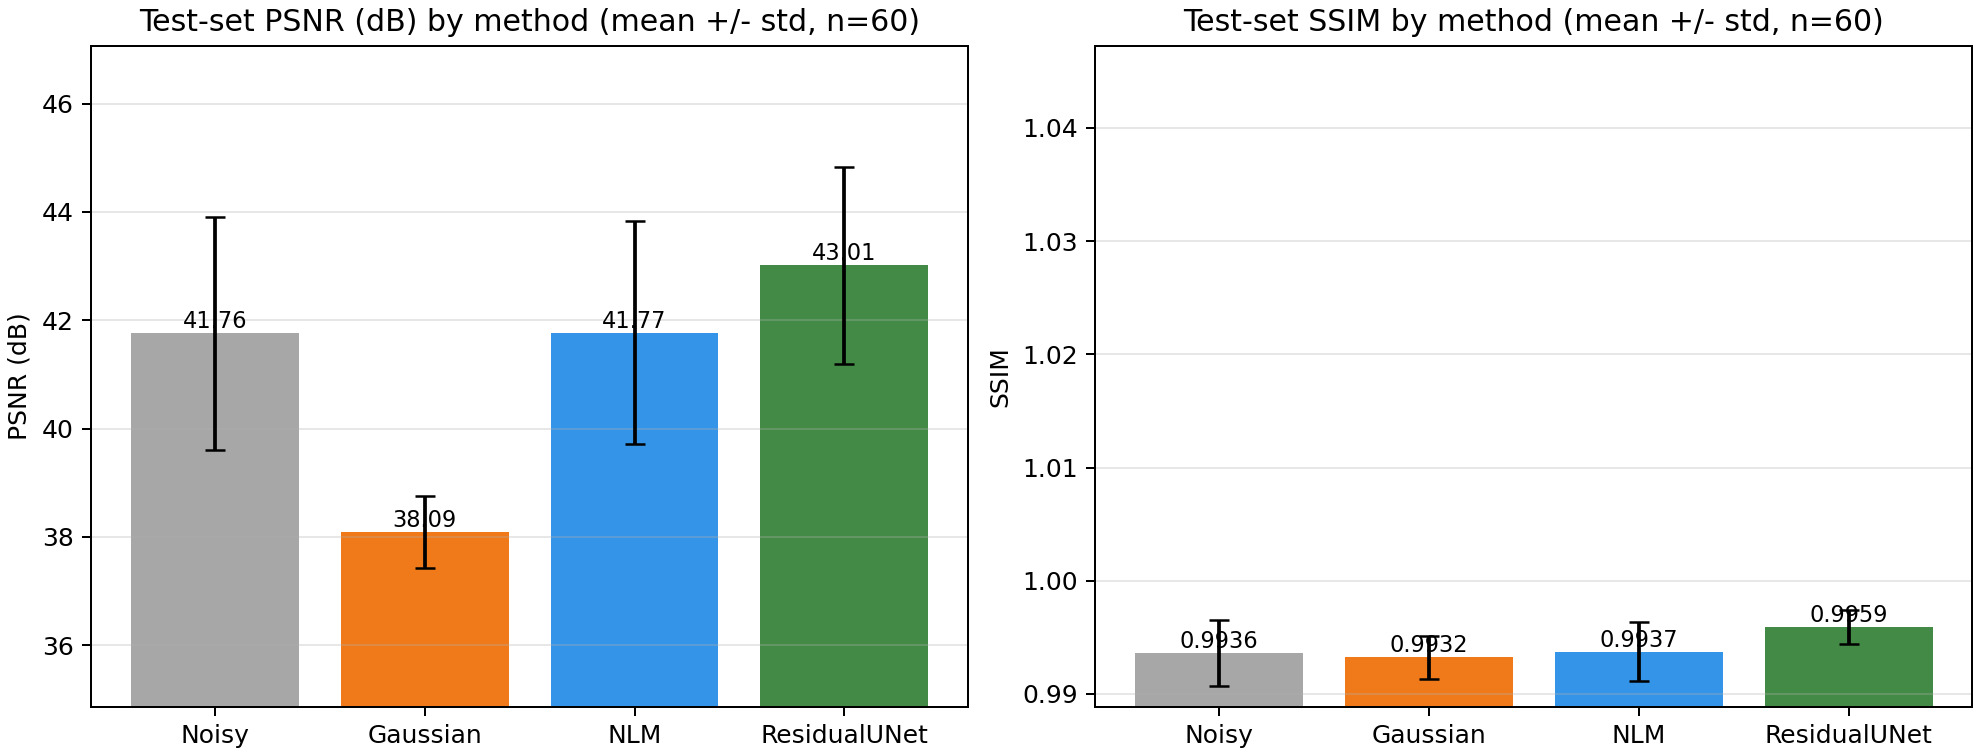
\includegraphics[width=0.92\linewidth]{fig_method_bars.png}
  \caption{不同方法的测试集指标对比。}
  \label{fig:bars}
\end{figure}

按 \texttt{rician\_sigma} 将测试病例分为低、中、高噪声三档，每档 20 例。Residual U-Net 在三档中均获得最高 PSNR。相对 Noisy 的 PSNR 增益从低噪声的 0.98 dB 增至高噪声的 1.52 dB，说明该模型在更强混合噪声下收益更明显。

\begin{table}[H]
  \centering
  \caption{按 Rician 噪声强度分层的 PSNR（dB, mean $\pm$ std）。}
  \label{tab:strata}
  \small
  \begin{tabular}{lccc}
    \toprule
    Method & Low noise & Mid noise & High noise \\
    \midrule
    Gaussian & $38.53\pm0.61$ & $38.17\pm0.43$ & $37.57\pm0.56$ \\
    NLM & $43.31\pm1.95$ & $41.82\pm1.40$ & $40.19\pm1.48$ \\
    Noisy & $43.41\pm2.05$ & $41.80\pm1.44$ & $40.09\pm1.52$ \\
    \textbf{Residual U-Net} & $\mathbf{44.39\pm1.77}$ & $\mathbf{43.04\pm1.20}$ & $\mathbf{41.61\pm1.27}$ \\
    \bottomrule
  \end{tabular}
\end{table}

\begin{figure}[H]
  \centering
  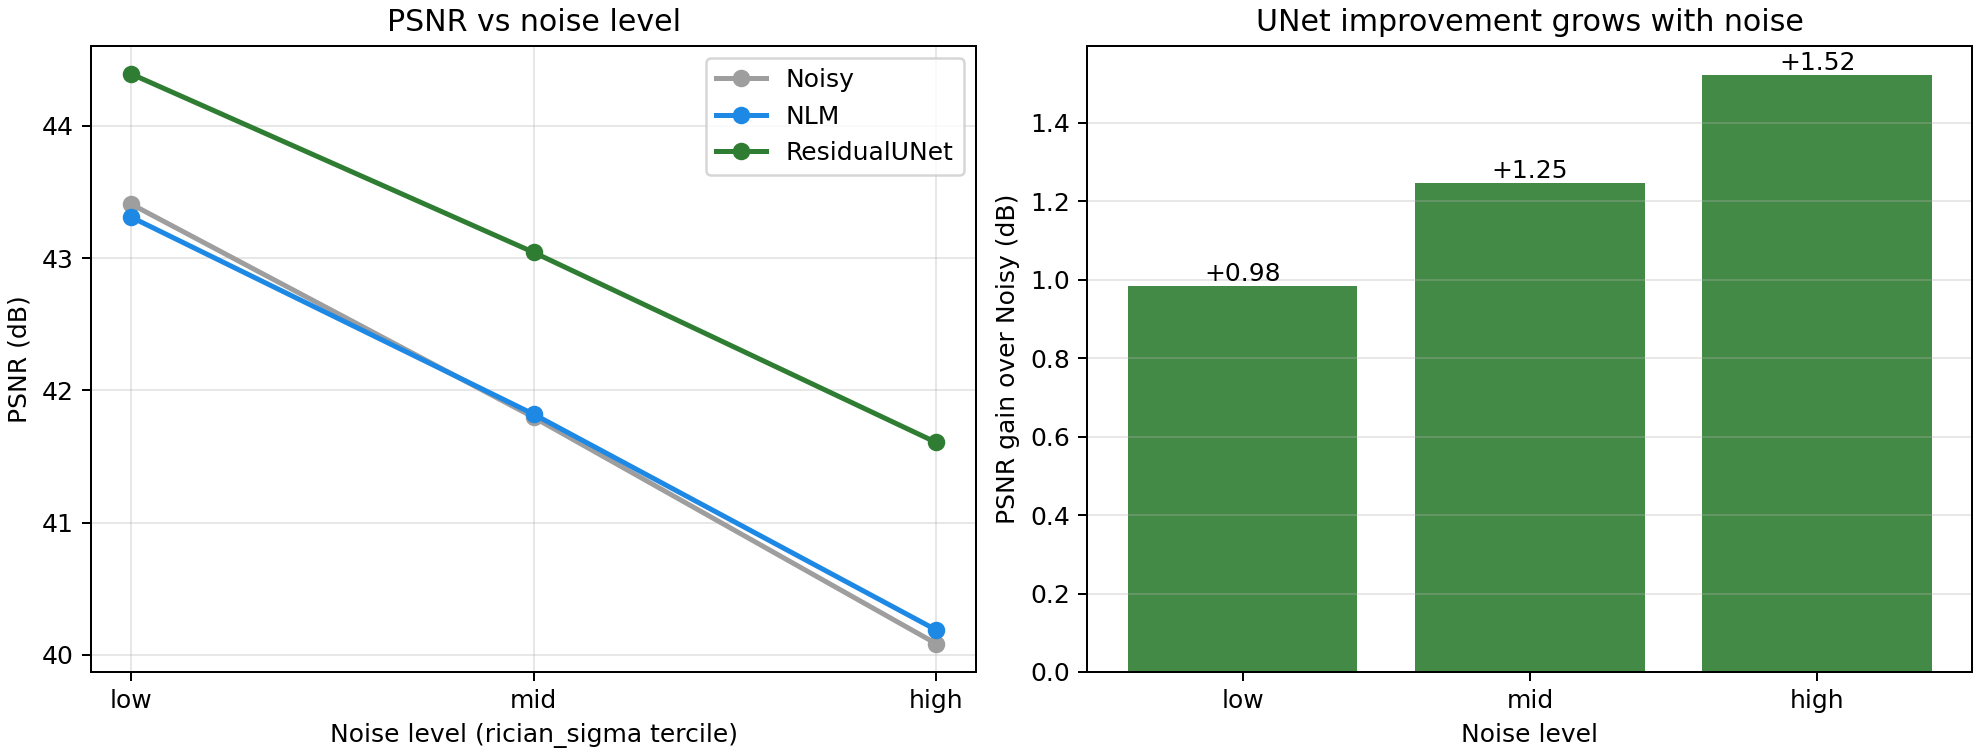
\includegraphics[width=0.82\linewidth]{fig_gain_vs_noise.png}
  \caption{Residual U-Net 相比 Noisy 的 PSNR 增益随噪声强度增加而增大。}
  \label{fig:gain}
\end{figure}

配对检验进一步支持该提升。Residual U-Net 在 60/60 个测试病例上 PSNR 均高于 Noisy、Gaussian 和 NLM。与 Noisy 相比，PSNR 平均差为 $+1.2508$ dB，配对 t 检验 $p=4.17\times10^{-35}$，Wilcoxon 符号秩检验 $p=1.63\times10^{-11}$。与 NLM 相比，PSNR 平均差为 $+1.2412$ dB，配对 t 检验 $p=2.06\times10^{-40}$。

\section{定性分析}

图~\ref{fig:qual_axial} 展示了高噪声测试病例 1051004 的 axial 切片。该病例中 Residual U-Net 相比 noisy 输入提升 1.96 dB PSNR。右侧两个误差图使用相同色标，显示 U-Net 输出相对 clean 的误差低于 noisy 输入，尤其是脑实质内部的随机误差明显减少。

\begin{figure}[H]
  \centering
  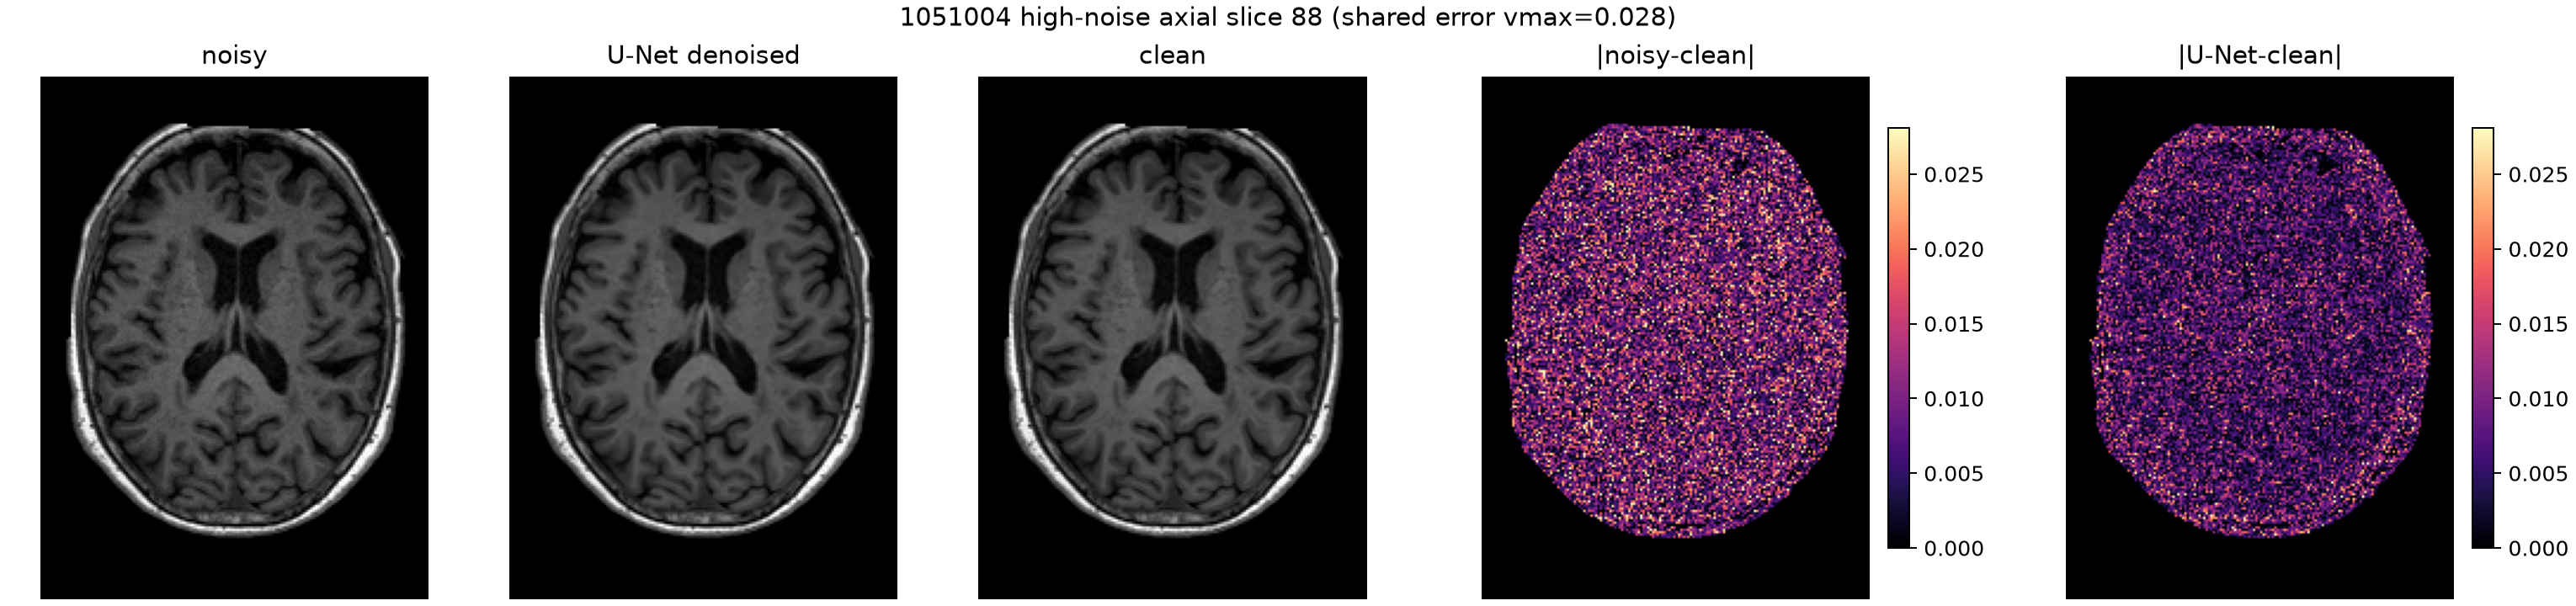
\includegraphics[width=\linewidth]{1051004_axial_compare.png}
  \caption{高噪声测试病例 1051004 的 axial 视图：noisy、Residual U-Net 输出、clean、noisy 误差与 U-Net 误差。两个误差图共享同一色标。}
  \label{fig:qual_axial}
\end{figure}

图~\ref{fig:qual_ortho} 给出了同一病例的 sagittal/coronal/axial 多平面视图。虽然模型按 axial 方向进行 2.5D 推理，重建体在其他平面上未见明显切片级断裂。

\begin{figure}[H]
  \centering
  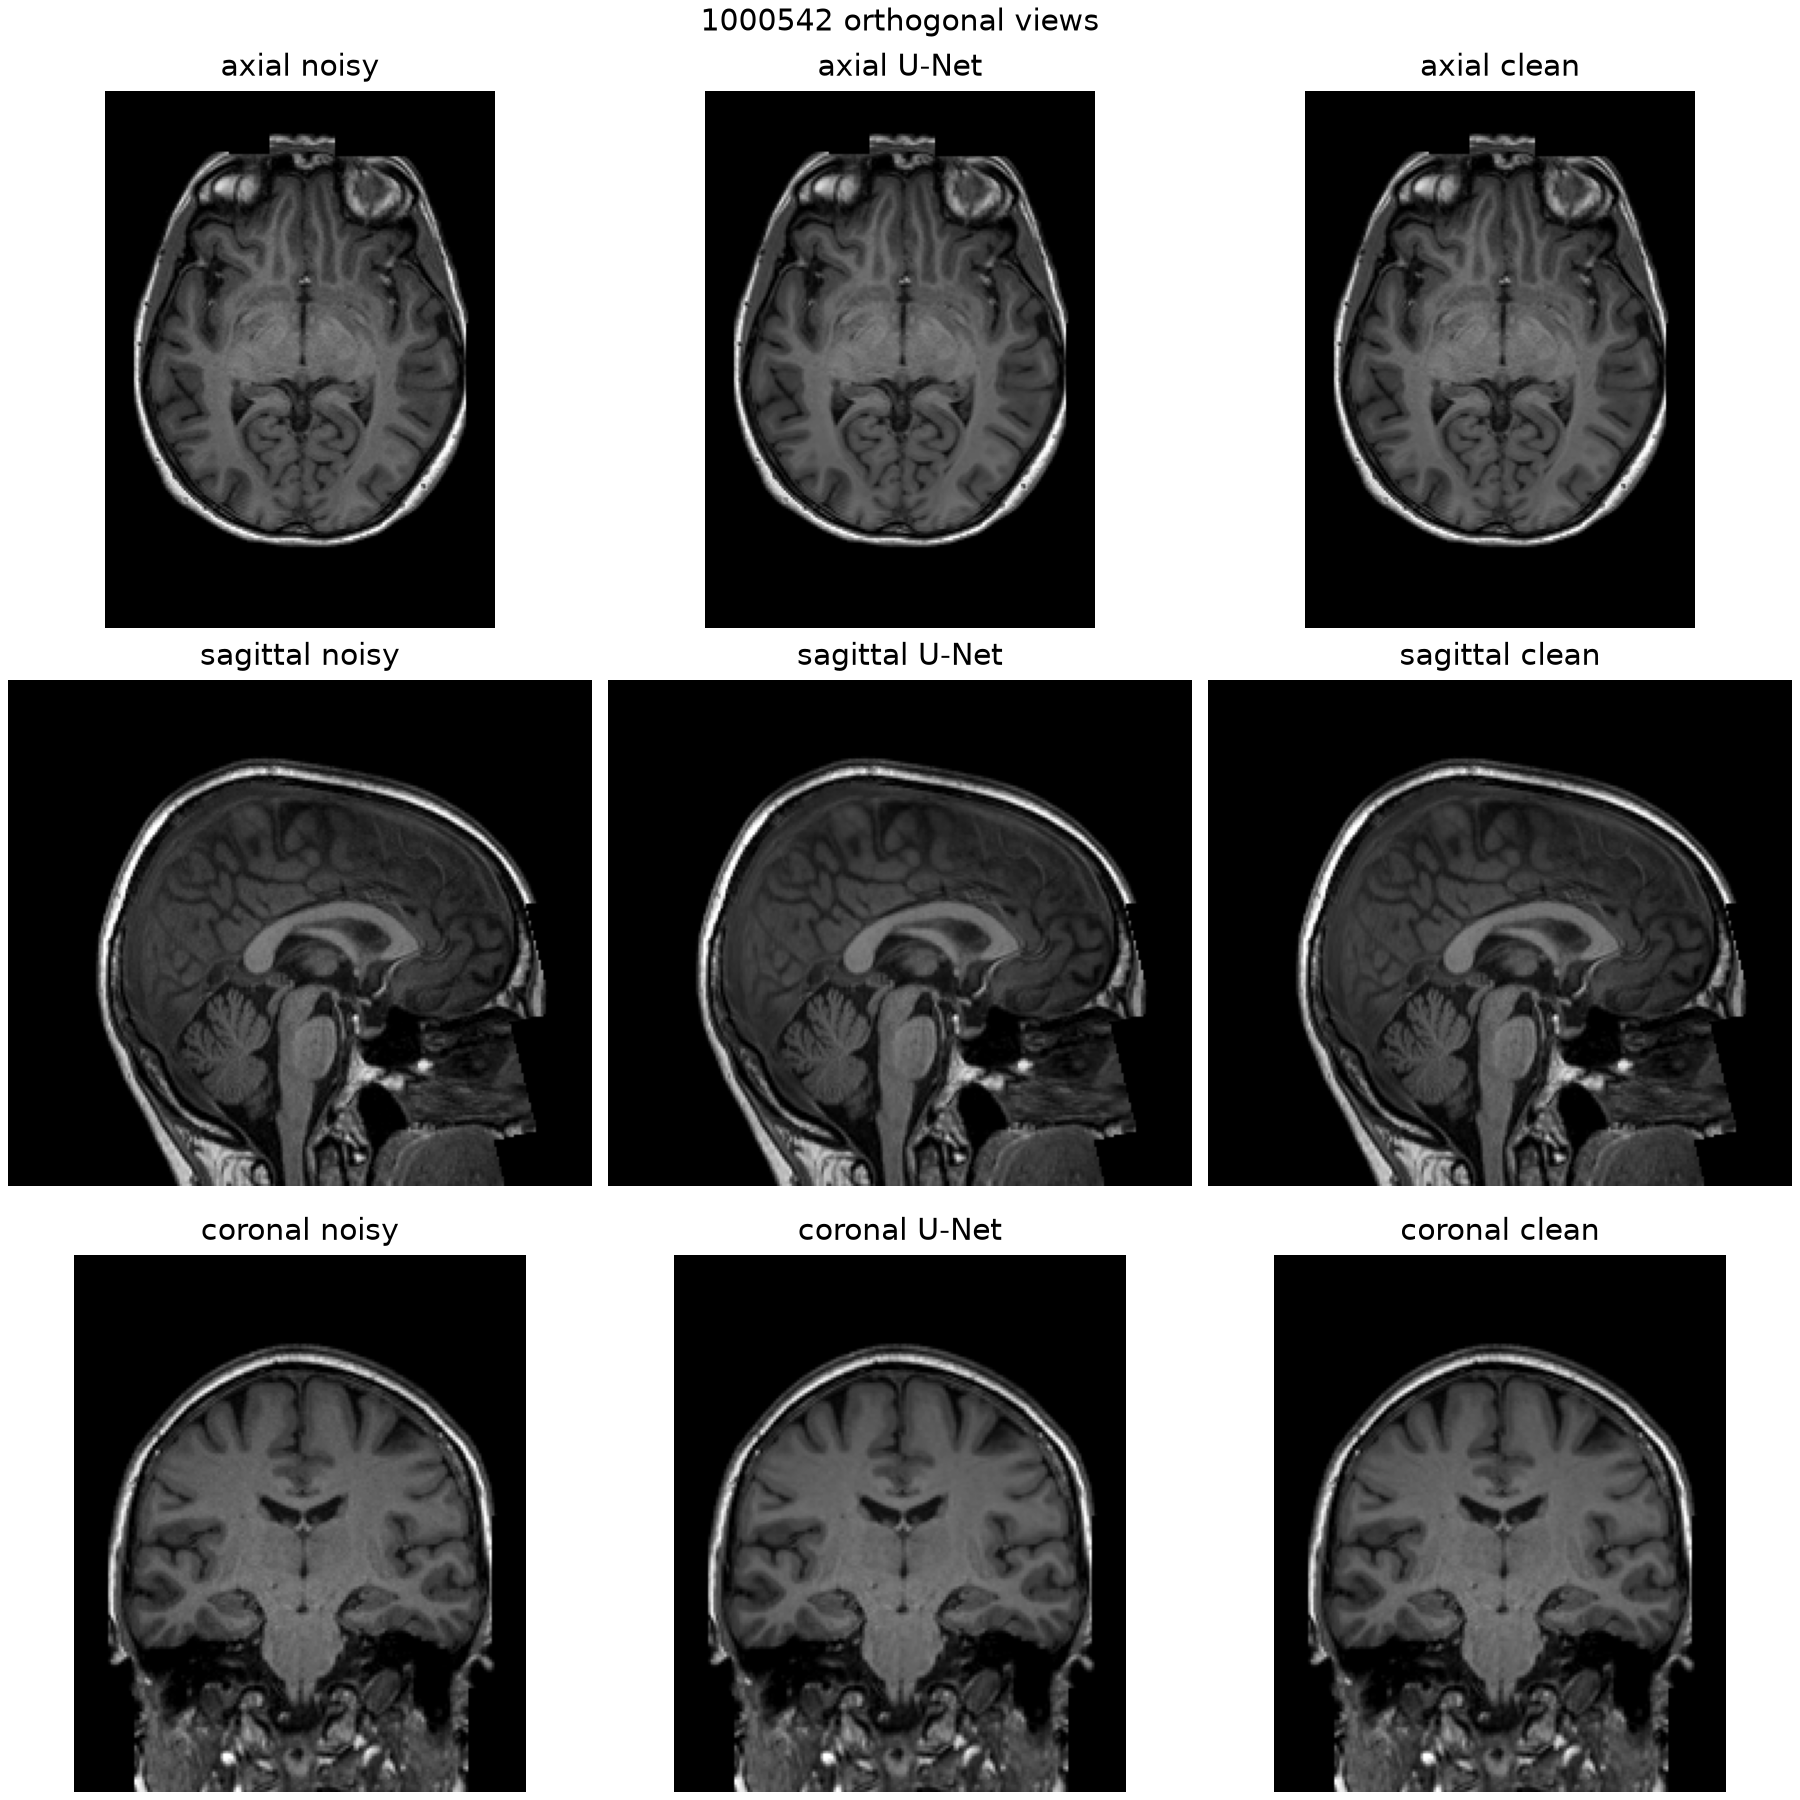
\includegraphics[width=\linewidth]{1000542_orthogonal.png}
  \caption{测试病例 1000542 的多平面可视化。}
  \label{fig:qual_ortho}
\end{figure}

\section{为何不继续训练}

本实验不再继续延长当前配置的训练。主要原因是模型已经到达 60 epoch，最佳验证结果出现在最后一个 epoch，但最后若干 epoch 的提升幅度很小。训练后期学习率已接近 0，验证 PSNR 从 epoch 53 的 43.0953 dB 到 epoch 60 的 43.0978 dB，仅提升约 0.0025 dB。这说明当前配置已基本进入平台期。

继续使用相同数据、相同模型和相同学习率计划训练，预期收益很低，并可能增加过拟合风险。若要进一步提升，优先方向应是新的实验设计，例如 3D 网络、模型集成、测试时增强或关键模块消融，而不是简单增加 epoch。

\section{结论}

本项目完成了可复现、可断点续传的 T1 MRI 去噪流程。主方法在测试集上达到 PSNR $43.01\pm1.82$ dB、SSIM $0.9959\pm0.0015$，并在所有测试病例上优于 Noisy、Gaussian smoothing 和 NLM。结果表明，2.5D 残差学习能在当前 Gaussian + Rician 混合噪声设置下稳定降低误差。当前实验的主要边界是：模型并非完整 3D 网络，结果基于单一病例级划分，且尚未在外部 MRI 数据上验证。

\end{document}
